%%% subsection
\section{Verification and Validation}
\label{sec:test_case}

\begin{figure}[ht]
    \centering
    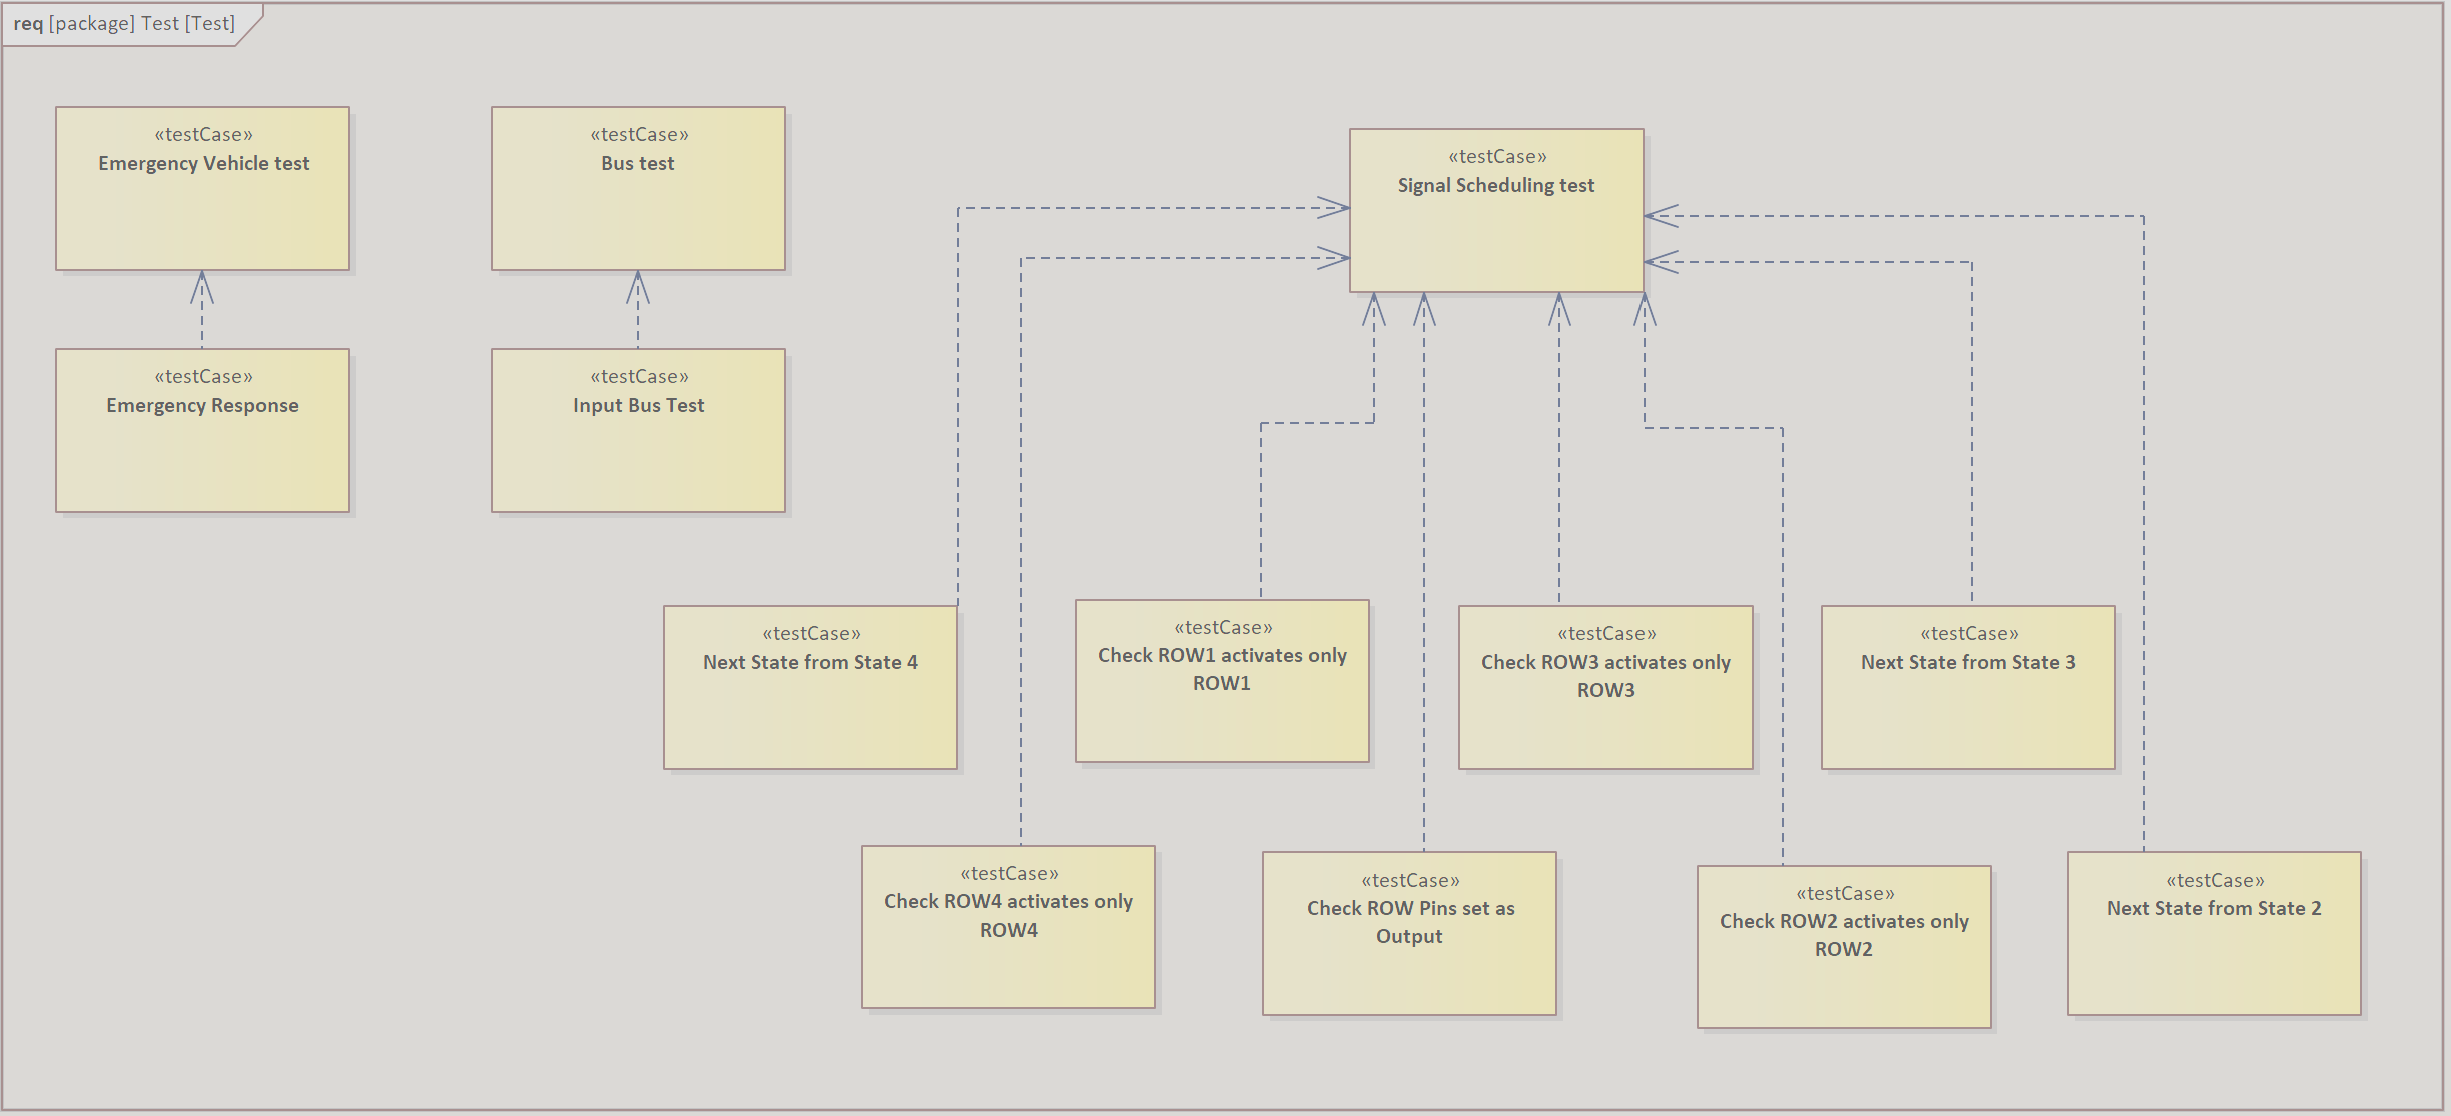
\includegraphics[width=0.5\textwidth]{images/test_case.png}
    \caption{Test case}
    \label{fig:picture1}
\end{figure}

This chapter describes the procedures and methodologies used during the device and defect testing phase of the signal scheduling system's V\&V process. The focus is on ensuring that the system meets design specifications and identifying any defects that may affect functionality, particularly in the areas of emergency response handling and signal scheduling.An overview of the test cases is illustrated in Figure \ref{fig:picture1}

In order to make sure that our system will work properly in an emergency vehicle, we made three tests:

\begin{enumerate}
    \item The first test verifies the ability of the system of processing into an emergency state or bus when a valid emergency signal is received. It ensures that the system will respond by entering the emergency state when an emergency signal or bus signal are received. The test confirms that the corresponding flag or state in the system is set to true, indicating that the system responds as expected.
    
    \item The second test is designed to assess the system's tolerance to invalid alarms. The alarm trigger is set to an unexpected value outside the range of valid alarms. The purpose of this test is to ensure that the system does not erroneously transition to an emergency state when invalid data is received. The test verifies that the \texttt{emergency\_state} remains false, demonstrating the system's capability to handle incorrect input signals without compromising its operational state.
    
    \item The purpose of third test is to validate the logic of the system's transition to a normal state after an alarm occurs. It evaluates whether the system can correctly transition to the next state when an emergency occurs. This is very important for scenarios where the system has to cancel the normal sequence of actions due to an emergency. The test ensures that the system continues to transition from one state to the next as required after an emergency.
\end{enumerate}

\subsection{Process 3: Signal Scheduler}
\label{subsec:signal_scheduler}

In order to test the signal scheduling system, we have written tests that check all the important functionality, detailed below:

\subsubsection{Next State from State Tests}
\label{subsubsec:next_state_from_state_tests}

These tests are designed to verify the logic that governs state transitions within the signal scheduling system. They confirm that the system correctly transitions from one state to the next in a predetermined sequence:
\begin{itemize}
    \item From state 1 to state 2,
    \item From state 2 to state 3,
    \item From state 3 to state 4, and
    \item From state 4 back to state 1.
\end{itemize}
Each test case focuses on a particular state transition, ensuring that the system's logic correctly handles the progression from one state to the next.

\begin{figure}[ht]
    \centering
    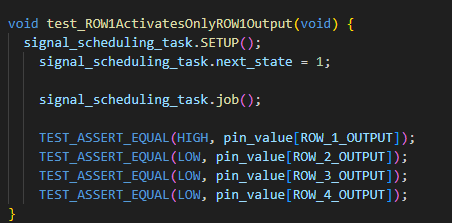
\includegraphics[width=0.4\textwidth]{images/screenshot_code_test.png}
    \caption{Testing ROW1 individually (sample code).}
    \label{fig:row1_test}
\end{figure}

\subsubsection{ROW Activation Tests}
\label{subsubsec:row_activation_tests}

Each of these test cases checks the individual activation of the ROW (Right of Way) outputs. They are designed to confirm that when a particular ROW, such as a traffic lane or signal light, is activated, only that specific ROW is active while all others remain inactive. This selective activation is crucial to prevent conflicting signals that could potentially lead to traffic problems. The procedure for these tests is exemplified in Figure \ref{fig:row1_test}

Similar tests are conducted for ROW2, ROW3, and ROW4, ensuring that each ROW's activation is handled correctly by the system.
